\documentclass[a4paper,11pt]{article}
%\pdfoutput=1 % if your are submitting a pdflatex (i.e. if you have
             % images in pdf, png or jpg format)
\usepackage{jheppub} % for details on the use of the package, please
                     % see the JHEP-author-manual
\usepackage[T1]{fontenc} % if needed


\usepackage{slashed}
%\usepackage{subfigure}
\usepackage{xspace}
\usepackage{booktabs}
\author[a]{Federico Ambrogi}

% e-mail addresses: one for each author, in the same order as the authors\emailAdd{federico.ambrogi@oeaw.ac.at}
\emailAdd{federico.ambrogi88@gmail.com}


%% %simple case: 2 authors, same institution
%% \author{A. Uthor}
%% \author{and A. Nother Author}
%% \affiliation{Institution,\\Address, Country}


\title{\boldmath Description of the script to extract humidities and dew points}
\begin{document} 
	\sffamily
	\maketitle


\section{Introduction}
All the scripts here described can be retrieved in \url{https://github.com/MBlaschek/CEUAS/tree/master/CEUAS/dev_federico/extract_Humidity_DewPoint}.
The aim is to analise the netCDF files, extracted from the odb files, regarding the relative humidity and dew point temperature. Whenever the data for these two variables is not available, the relative humidity will be calculated using the temperature and the dew point temperature. In principle it is possible to calculate relative humidity by using the specific humidity and the temperature, however this method results in unclear discrepancy, as it will be shown in Section \ref{comparison}.

\section{Description}
The script \verb|extract_Humidity_Temperature.py| reads the data contained in the files for temperature, humidity (specific and relative), and dew point temperature for a given observation station. The first element to check is that the datum available for each variable, i.e. the array of observation dates, is identical, since in principles they can be different. For example, some entries might be missing. In general the temperature data should always be present, and it is needed in order to extract the others. 
\\

The script then checks if the values of the relative humidity and dew points are available. If such values are available, there is nothing to be done. Otherwise, a new file called "\_calc\_sh\_rh\_dp.nc" is produced, containing a merged dataset with the original observation data, and calculated values for the missing entries. According to the \textbf{CDM} conventions, the variables are named "\textit{dew\_point\_temperatures}", "\textit{relative\_humidity}" and "\textit{specific\_humidity}". 
\\
To keep a record of the source of the data, an additional field with a prefix 'source\_' plus the name of the variable is added to the file. For each entry, the value '1' is assigned to observation data (or data from the odb file), and '2' to calculated values. 
\\
The functions used for the conversion of the variables are defined in the script called "humidity" . 



\section{FOEEWMO vs sh2rh} \label{comparison}
The \textbf{FOEEWMO} and \textbf{sh2rh} function allow for the calculation of the relative humidity, starting respectively from the dew point temperature and the specific humidity. The definition of such functions can be find in the document ECMWF IFS CY31R1 Data Assimilation Documentation (Page 86-88) at \url{https://www.ecmwf.int/en/elibrary/9225-part-ii-data-assimilation} .
The values of the relative humidity calculated with the two functions were tested against the observed data for the station 10393, since both the specific and relative humidity and the dew point temperature are available. Fig. \ref{ratio} shows that, while the FOEEWMO function reproduces accurately the values of the observed relative humidity, the function sh2rh gives a constant offsett of 0.62 . This is still under investigation.


\begin{figure}[!b]
	\centering
	\subfigure
	{ 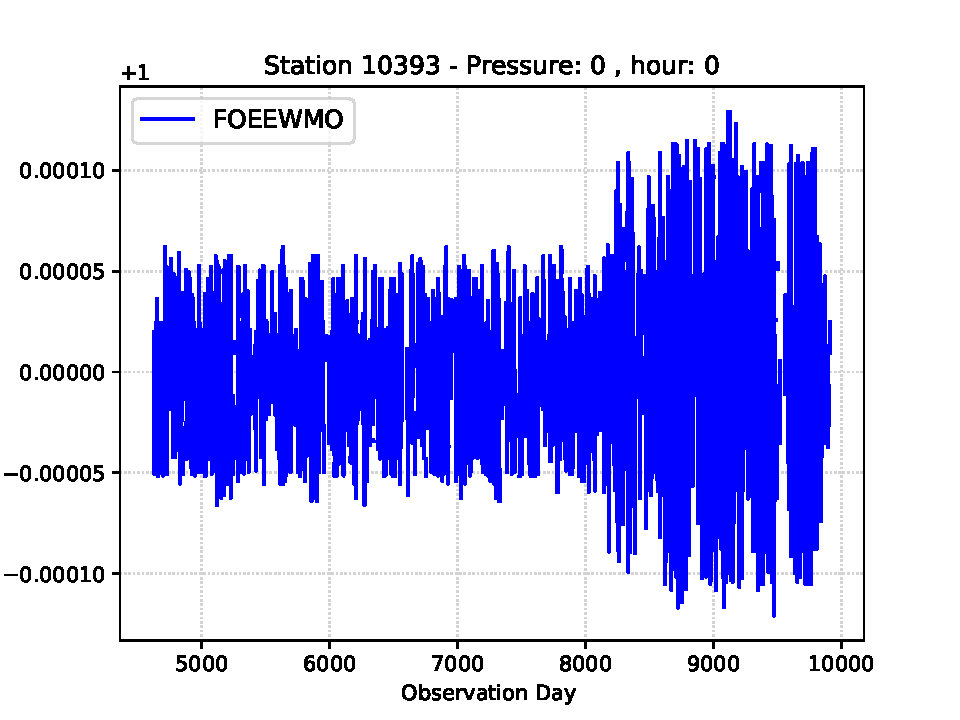
\includegraphics[width=0.49\textwidth]{Fig/ratios_FOEEWMO_0_0.pdf}}
	\subfigure
	{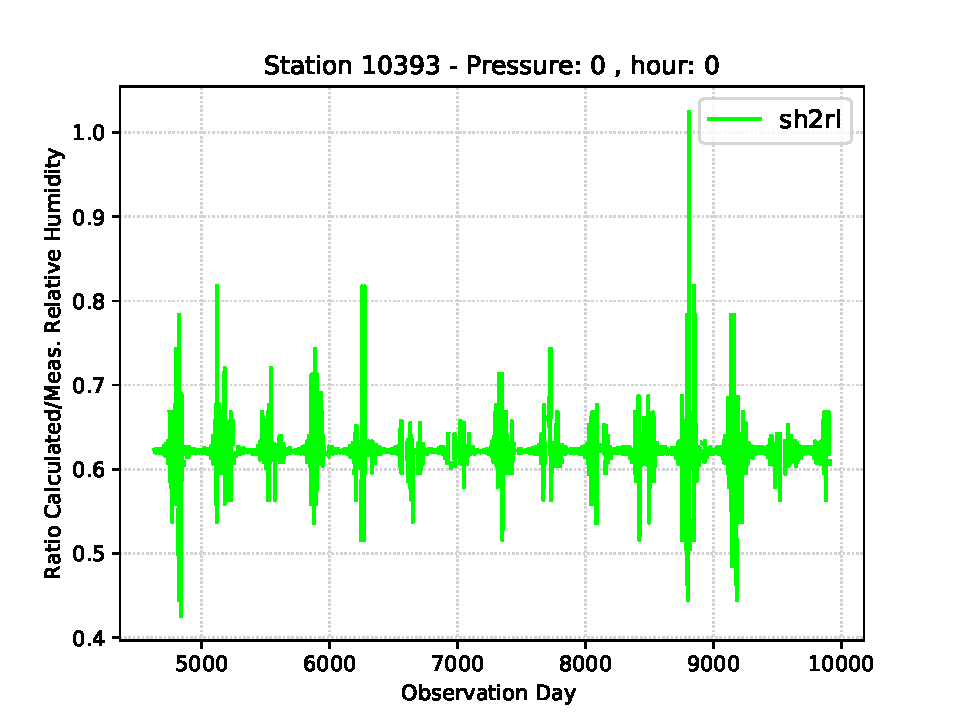
\includegraphics[width=0.49\textwidth]{Fig/ratios_sh2rl_0_0.pdf}}
	\caption{Ratio of the calculated versus observed relative humidity, using the FOEEWMO (left) and sp2rh (right) functions.}
	\label{ratio}
\end{figure}
	





\end{document}



